\item \begin{theorem}{(371)} 只有\code{jump}和\code{MemtoReg}上面$1$下面$0$,其他皆相反。
    \begin{figure}[H]
        \centering
        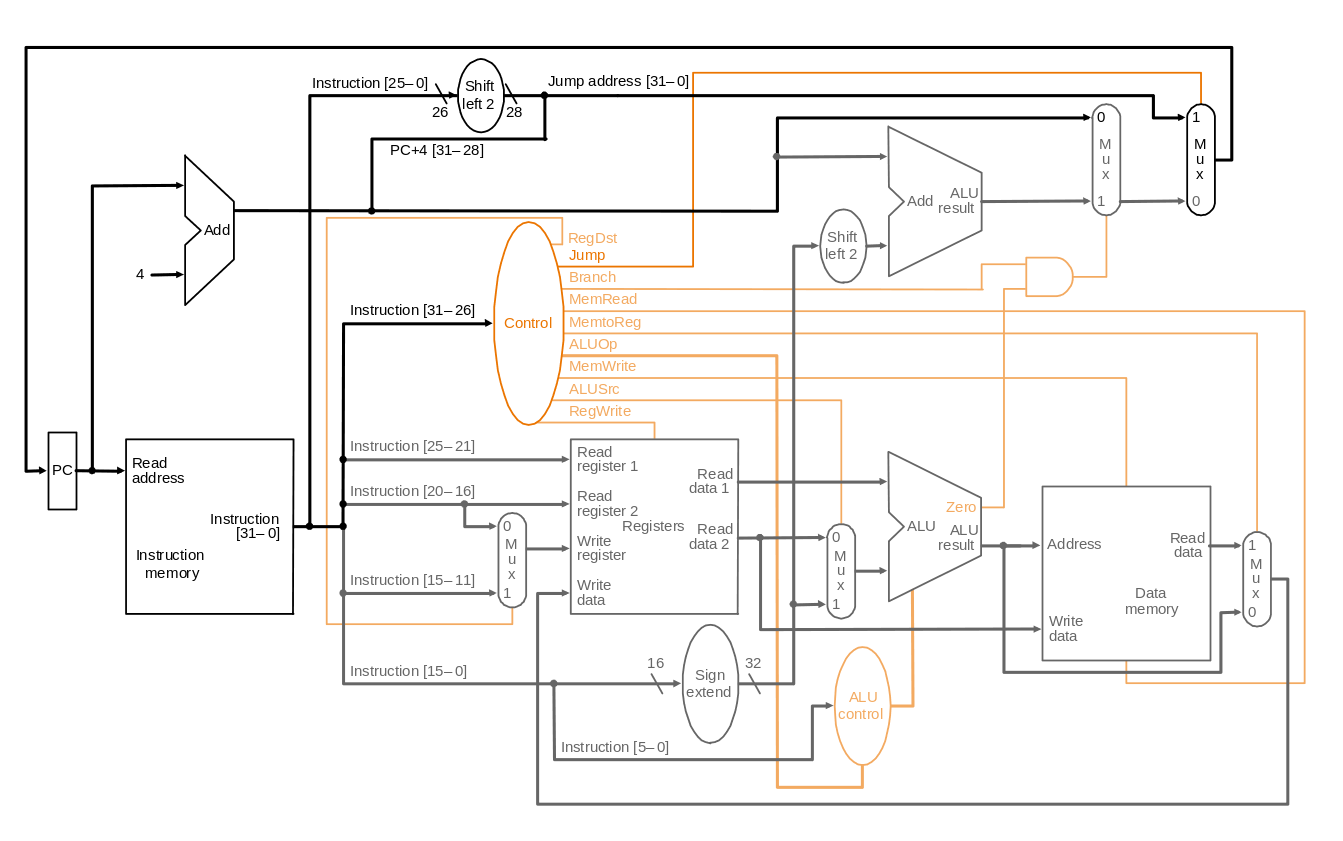
\includegraphics[scale=0.3]{img/single-cycle-cpu.png}
        \caption{Single-cycle CPU with jump and branch.}
        \label{img:single-cycle-cpu}
    \end{figure}
\end{theorem}

\item \begin{theorem}{(384)} \quad\quad
    \begin{table}[H]
        \centering
        \begin{tabular}{|c|c|c|}
            \hline
            Instruction & ALUOp1 & ALUOp2 \\
            \Xhline{2\arrayrulewidth}
            \code{lw/sw} & $0$ & $0$ \\
            \hline
            \code{beq} & $\texttimes$ & $1$ \\
            \hline
            R-type & $1$ & $\texttimes$\\
            \hline
        \end{tabular}
    \end{table}
\end{theorem}
